%!TEX root = ../tesis.tex
\section{Motivaci\'on}
\label{sec:motivacion}

La habilidad de producir y entender el lenguaje oral ha sido se\~nalada por los antrop\'ologos
como uno de los principales logros de nuestra especie. Varios investigadores coinciden
en considerar el lenguaje como un instinto, una adaptaci\'on biol\'ogica que nos permite
comunicar \mbox{informaci\'on \cite{GabrielVoice2007}}.

Habiendo establecido la importancia del habla, resulta natural pensar en formas de
interactuar con las computadoras a trav\'es de la misma.

De acuerdo a los reportes de la renombrada consultora tecnol\'ogica Gartner, el reconocimiento
del habla alcanzara la  \emph{meseta de la productividad} en los pr\'oximos 2 a 5 a\~nos. Esto es,
se convertir\'a en una tecnolog{\'\i}a estable y cuyos beneficios est\'an ampliamente demostrados
y \mbox{aceptados \cite{Gartner2013}}.

\begin{figure}[ht]
\centering
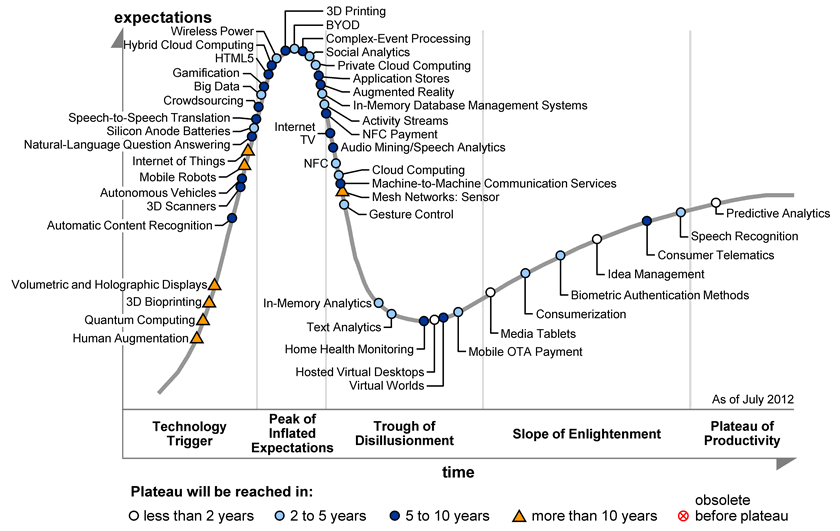
\includegraphics[width=0.8\linewidth]{./graphics/gartner.png}
\caption{Ciclo de Sobreexpectaci\'on de tecnolog{\'\i}as emergentes de \mbox{Gartner -- 2013 \cite{Gartner2013}.}}
\label{figure:gartner}
\end{figure}
%Figura Gartner

El dise\~no y la implementaci\'on de una interfaz mediante voz del usuario representa
una oportunidad, no solo para el estudio de esta \'area de investigaci\'on, sino para
demostrar la aplicabilidad del reconocimiento del habla a un problema real.

Habiendo mencionado previamente la potencial importancia del dominio de la aplicaci\'on
para una interfaz por voz del usuario, la elecci\'on de un programa de composici\'on musical
no pod{\'\i}a ser injustificada.
Existen investigaciones realizadas que relacionan a la m\'usica y el reconocimiento
del habla, en particular, orientadas al problema de recuperaci\'on de informaci\'on
\mbox{musical \cite{Goto2004Speech, Schuller2003Hybrid}}.
Sin embargo, resulta interesante experimentar con la utilizaci\'on del reconocimiento
del habla para la composici\'on musical. Este enfoque, en el cual un programa recibe comandos
sonoros y emite tambi\'en un resultado sonoro, podr{\'\i}a resultar incluso m\'as natural.

El programa de composici\'on musical controlado por voz es un medio para:

\begin{itemize}
	\item Explorar y experimentar con el reconocimiento del habla y las interfaces de usuario.
	\item Contrastar teor{\'\i}a y pr\'actica.
	\item Demostrar la factibilidad de la soluci\'on de un problema real utilizando el
	reconocimiento del habla.
\end{itemize}